\chapter{Mathematisch korrektes WG-Casting}
\label{WG-Casting}

\section{Mitbewohner*in gesucht!}
Emmy, Maryam, Carl und Bertrand wohnen zusammen in einer WG in der Weierstraße 2. Seit Kurt ausgezogen ist, suchen sie eine*n neue*n Mitbewohner*in für das freigewordene Zimmer. Nach ihrer Anzeige auf chillig-und-billig.de melden sich binnen kürzester Zeit viele Interessent*innen - so viele, dass Emmy, Maryam, Carl und Bertrand sich nach 17 Minuten und 73 Bewerbungen entscheiden, die Anzeige wieder von der Seite zu nehmen. Sie beschließen, mit den vorhandenen Bewerber*innen ein WG-Casting durchzuführen, um den*die optimale*n Mitbewohner*in zu bestimmen.
\begin{center}
	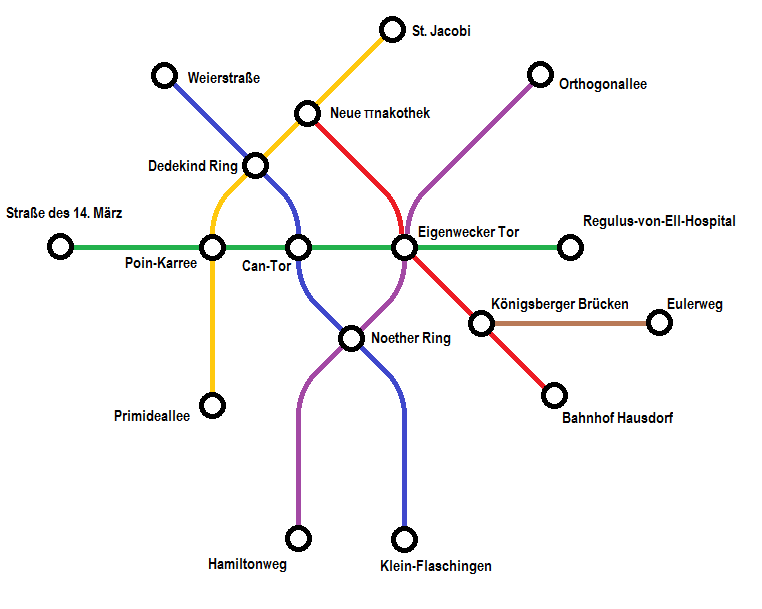
\includegraphics{images/wg/ubahn.png}
\end{center}
Alle sind sich einig, dass das hervorstechendste Merkmal eines guten Mitbewohners sein sollte, dass er oder sie gerne scharfes Essen isst - je schärfer, desto besser. Beim WG-Casting soll nun deshalb jede*r Bewerber*in unauffällig auf die Probe gestellt werden. Die schärferesistenteste Person soll das Zimmer bekommen.

Die Regeln von chillig-und-billig.de fordern, dass man einem*r Bewerber*in nach dem Casting sofort zu- oder absagen muss. Die Betreiber der Seite begründen das folgendermaßen: "Nach einem Casting lange auf eine Rückmeldung zu warten erschwert Bewerber*innen die Planung und damit die Wohnungssuche. Wer sich bewirbt und zu einem Casting geht, soll auch schnell eine Antwort bekommen. Denn Zeit ist nicht billig und Warten ist unchillig." Emmy, Maryam, Carl und Bertrand können also nicht erst alle 73 Bewerber*innen begutachten und danach eine Entscheidung treffen. Stattdessen müssen sie nach jedem Casting entscheiden, ob sie die Person nehmen oder nicht. Erst nach einer Absage bekommen sie die nächste Person zum Casting zugeteilt.

Um garantiert eine optimale Entscheidung zu treffen, müsste man die Zukunft voraussehen können. Aber es kann ja niemand wissen, ob nach einer bestimmten Person noch eine bessere kommt oder nicht. Deshalb müssen Emmy, Maryam, Carl und Bertrand probabilistisch vorgehen: Was wäre eine gute Casting-Strategie, um mit möglichst hoher Wahrscheinlichkeit den*die beste*n Kandidat*in zu wählen?

\begin{center}
	
\includegraphics{images/wg/zukunft.png}
\end{center}
Abb. 1: Niemand kann die Zukunft voraussehen.

Quellen:

Abb. 1: Bild \href{https://pixabay.com/de/illustrations/zukunft-kristallkugel-vorhersage-1126760/}{zukunft-kristallkugel-vorhersage} von \href{https://pixabay.com/de/users/rilsonav-1824615/}{Rilsonav}, \href{https://pixabay.com/de/service/terms/}{Pixabay License}, via Pixabay

\section{Erste Casting-Strategien}
Die vier diskutieren, wie sie am besten vorgehen sollten. Um die Ergebnisse für zukünftige WG-Castings nutzen zu können, stellen sie ihre Überlegungen für eine allgemeine Anzahl von $N$ Bewerber*innen an.

Bertrand hat eine Idee: "Lass doch einfach den ersten Bewerber nehmen. Erinnert ihr euch noch an diese Multiple-Choice Klausur letztes Semester? Da war auch die erste Option immer die richtige."

Die vier überlegen und kommen zu folgendem Ergebnis: Die Wahrscheinlichkeit, dass sich die schärferesistenteste Person ausgerechnet auf der ersten Position in der Liste der $N$ Bewerber*innen befindet, beträgt genau
\[
	P=\frac{\text{Anzahl beste Personen}}{\text{Anzahl Bewerbungen}}=\frac{1}{N}.
\]
Bei einer großen Zahl Bewerbungen ist es mit dieser Methode nicht besonders wahrscheinlich, die beste Person zu erwischen. Zum Beispiel würde die Erfolgswahrscheinlichkeit bei $N=73$ Bewerbungen nur $\frac{1}{73}\approx 1{,}4\,\%$ betragen. Das ist nicht besonders viel.

Carl widerspricht dem Argument, dass die erste Option immer die beste sei: "Das war vielleicht in der Klausur so, aber bei Entscheidungen, wo es wirklich um was geht, soll man nie die erstbeste Option nehmen. Das weiß doch jeder! Lehnen wir doch den ersten Bewerber nach dem Casting einfach ab und nehmen den zweiten."

Es dauert nicht lang, bis die vier die Erfolgswahrscheinlichkeit der von Carl vorgeschlagenen Methode ermittelt haben: Die Wahrscheinlichkeit, dass sich die beste Person auf Platz 2 in der Liste der $N$ Bewerber*innen befindet, beträgt ebenfalls nur $P=\frac{1}{N}$.

Auch nach Emmys Vorschlag, "Die Antwort auf Alles ist 42. Was, wenn wir einfach immer den 42. nehmen?", müssen die vier feststellen, dass die Wahrscheinlichkeit, auf diese Weise den*die beste*n Bewerber*in zu wählen, genau dieselbe ist: $P=\frac{1}{N}$.

"Ja nee", wirft Bertrand ein, "wenn wir jetzt schon ausmachen, nach dem*der wievielten Bewerber*in wir das Casting beenden, dann kriegen wir ja immer mit der gleichen Wahrscheinlichkeit den*die Beste*n. Dann können wir uns die Castings auch sparen und wirklich einfach den ersten nehmen!"

Maryam verliert die Geduld: "Ey Leute, ich glaub nicht, dass das zu was führt. Das muss doch noch besser gehen. Wir müssen mehr out of the box denken."

\section{Die bessere Strategie}
Maryam fährt fort: "Ich stimme Carl zu, dass wir nicht den*die erstbeste*n Bewerber*in nehmen sollten. Die Erfolgswahrscheinlichkeit ist viel zu gering. Aber wenn wir den*die erste*n Bewerber*in nach dem Casting ablehnen, will ich danach keinen nehmen, der*die schlechter als der*die Erste ist. Das wär ganz schön blöd."

"Ja stimmt", meint Carl. "Dann nehmen wir halt danach den*die Nächste*n, der*die besser ist als der*die Erste."

"Wenn wir so vorgehen, sollten wir aber erst einen besseren Eindruck haben, wie die Bewerber*innen überhaupt sind", gibt Emmy zu bedenken. "Ich bin dafür, dass wir anfangs noch mehr Leute ablehnen, bevor wir jemanden auswählen. Bewerbungen haben wir ja genug."

Alle finden diesen Vorschlag gut. Die vier beschließen, sich erst eine gewisse Anzahl $r$ an Bewerber*innen anzuschauen und abzulehnen. Danach interviewen sie den Rest und nehmen die nächste Person, die besser als die ersten $r$ Bewerber*innen ist.
\begin{center}
	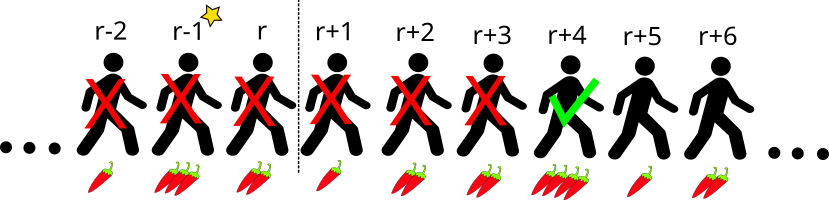
\includegraphics{images/wg/bewerber.svg}
	Person r-1 war die beste unter den ersten r, die abgelehnt wurden. Danach ist Person r+4 die erste, die besser ist, und wird deshalb ausgewählt.
\end{center}
Nur Bertrand macht sich noch Sorgen: "Aber je mehr wir am Anfang ablehnen, desto größer ist doch die Wahrscheinlichkeit, dass sich die beste Person unter den bereits abgelehnten Personen befindet! Wie soll das funktionieren?"

"Wir müssen einfach nur $r$ klug wählen", meint Emmy. "Dann wird das schon passen."

"Dann sag doch mal, wie wir $r$ 'klug' wählen können", fordert Bertrand. Unter den erwartungsvollen Blicken der anderen sucht sich Emmy Papier und einen Bleistift und beginnt zu rechnen.

\section{Mathematische Untersuchung der Strategie}
Die Strategie der vier ist, die ersten $r$ der NNN Bewerber*innen abzulehnen und danach die erste Person zu nehmen, die besser als die ersten $r$ Bewerber*innen ist. Emmy will nun $r$ so wählen, dass die Wahrscheinlichkeit $P\left(r\right)$, mit dieser Strategie die beste Person zu finden, maximal ist. Dafür muss sie $P\left(r\right)$ in Abhängigkeit von $r$ berechnen. 
\begin{verstaendnisfrageQuery}
	Wann wird denn mit dieser Strategie nicht die beste Person ausgewählt?
\end{verstaendnisfrageQuery}
\begin{antwort}
	Wenn die*der beste Bewerber*in unter den ersten $r$ Personen ist, wählt man mit dieser Strategie die letzte Person aus. In dem Fall können wir nicht die beste Person auswählen.
	
	Aber selbst wenn die beste Bewerbung nicht unter den ersten $r$ Bewerber*innen ist, kann die Strategie scheitern. Angenommen, die beste Bewerbung ist Person $r+2$ und die zweitbeste ist Person $r+1$. Dann wählen wir Person $r+1$, weil sie sicherlich besser ist als die ersten $r$ Bewerber*innen. So haben wir aber nicht die beste Person, nämlich Person $r+2$ ausgewählt.
	
	Die beste Person wird also nicht ausgewählt, wenn sie unter den ersten $r$ ist oder eine Person, die früher kommt als sie, besser als die ersten $r$ ist. 
\end{antwort}
Emmy geht die einzelnen Kandidat*innen nach den ersten $r$ Leuten durch und berechnet jeweils die Wahrscheinlichkeit, dass die Person die beste Wahl ist und sie mit der Strategie ausgewählt wird. 
\begin{box}
	\emph{$r+1$ste Person}
	
	Was ist die Wahrscheinlichkeit, dass sie die beste Wahl ist und sie mit der Strategie ausgewählt wird?
	
	Die Wahrscheinlichkeit, dass sie die beste Person ist, ist wieder $\frac 1N$​.
	
	Weil sie die beste Person ist, ist sie auch besser als die ersten $r$ Personen. Weil sie direkt nach den abgelehnten $r$ Personen kommt und besser als sie ist, wird sie auch ausgewählt. Also ist die Wahrscheinlichkeit, dass sie ausgewählt wird, $1$.
	
	Insgesamt ist die Wahrscheinlichkeit, dass die $r+1$ste Person die beste ist und ausgewählt wird, gleich $\frac{1}{N}\cdot 1=\frac{1}{N}$​.
\end{box}
Wie sieht es mit der nächsten Bewerbung aus?
\begin{box}

	\emph{$r+2$te Person}

	Was ist die Wahrscheinlichkeit, dass sie die beste Wahl ist und sie mit der Strategie ausgewählt wird?

	Dass Person $r+2$ die beste ist, gilt mit einer Wahrscheinlichkeit von $\frac 1N$​.

	Wir wählen Person $r+2$ genau dann aus, wenn der*die Bewerber*in $r+1$ nicht besser war als die ersten $r$ Personen. Mit welcher Wahrscheinlichkeit ist Person $r+1$ besser als die ersten $r$ Bewerber*innen? Das ist der Fall, wenn die beste Person aus den Bewerber*innen $1,\ldots, r+1$ Person $r+1$ ist. Das gilt mit einer Wahrscheinlichkeit von $\frac 1{r+1}$​.

	Unsere gesuchte Wahrscheinlichkeit ist also
	\[ 1-\frac 1{r+1}=\frac r{r+1}.\]

	Insgesamt ist die Wahrscheinlichkeit dafür, dass die $r+2$te Person die beste ist und mit dieser Strategie ausgewählt wird, gleich $\frac1N\cdot\frac{r}{r+1}$.
\end{box}
Was gilt allgemeiner für die $i$te Person, die nach den ersten $r$ kommt?
\begin{box}
	\emph{$i$te Person mit $i>r$}
	
	Was ist die Wahrscheinlichkeit, dass sie die beste Wahl ist und sie mit der Strategie ausgewählt wird?
	
	Die Person $i$ ist die beste mit einer Wahrscheinlichkeit von $\frac 1N$​.
	
	Wir wählen sie genau dann aus, wenn die Personen $r+1, \ldots , i-1$ nicht besser sind als die beste der ersten $r$ Personen. Mit welcher Wahrscheinlichkeit ist keine der Personen $r+1,\ldots,i-1$ besser als die ersten $r$ Personen? Das gilt genau dann, wenn die beste der ersten $i-1$ Personen eine der Personen $1,\ldots,r$ ist. Die Wahrscheinlichkeit dafür ist
	\[\frac r{i-1}.\]
	
	Insgesamt ist die Wahrscheinlichkeit, dass die $i$te Person die beste Wahl ist und mit der Strategie ausgewählt wird, gleich $\frac1N\cdot \frac{r}{i-1}$​.
\end{box}
Die Gesamtwahrscheinlichkeit, mit der Strategie die beste Person auszuwählen, ist die Summe der einzelnen Wahrscheinlichkeiten für die einzelnen Personen:
\[P=P(r)=\sum_{i=r+1}^N\frac{1}{N}\cdot\frac{r}{i-1}\]
Emmy präsentiert die Wahrscheinlichkeit stolz ihren Freunden.

Bertrand ist noch nicht zufrieden. "Wie sollen wir nun das richtige $r$ finden, für das $P(r)$ maximal ist?", fragt er.

"Das ist ja einfach eine Extremwertaufgabe", meint Carl, "ich weiß, wie das geht, da muss man die Ableitung von $P(r)$ finden und herausfinden, für welches $r$ die Ableitung Null ist!"

"Wie willst du denn bitte diese Funktion nach $r$ ableiten?!", entgegnet Maryam. "Siehst du nicht, dass auch der Index der Summe von $r$ abhängt?"

"Ich hab da eine Idee", meint Emmy. "Wir können die Summe durch ein Integral abschätzen."
\[P(r)=\sum_{i=r+1}^N\frac{1}{N}\cdot\frac{r}{i-1}\approx\frac{1}{N}\int_{r+1}^{N+1}\frac{r}{x-1}\mathrm{dx}\]
"Die Summe ist dann die linke Riemannsumme des Integrals", erklärt Emmy. 
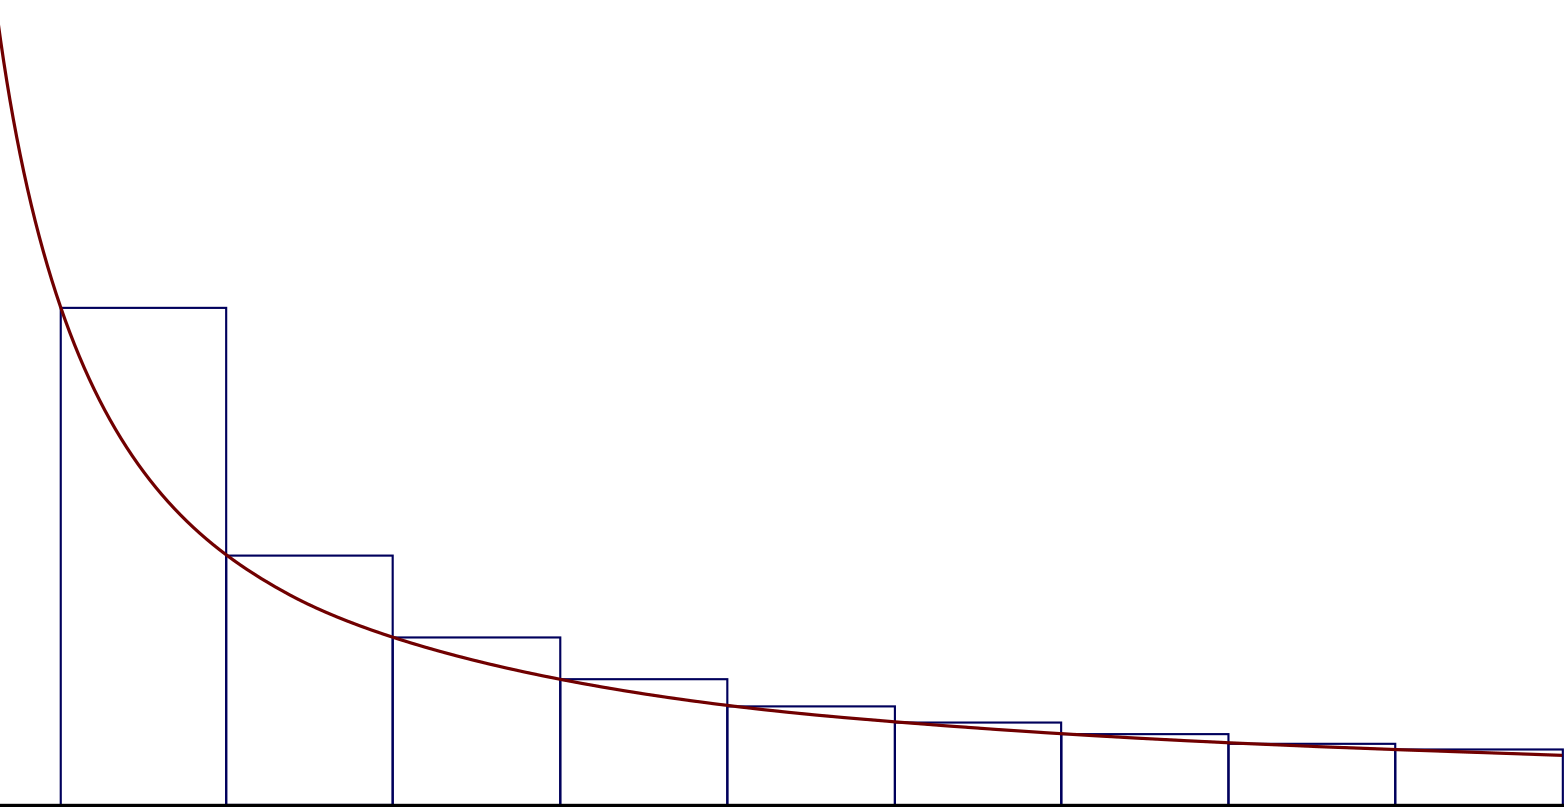
\includegraphics{images/wg/integral.png}
Abb.1: Linke Riemannsumme der Funktion $\frac{1}{x}$

"Das Integral können wir ganz leicht berechnen", fährt Emmy fort. 
\[\frac{1}{N}\int_{r+1}^{N+1}\frac{r}{x-1}\mathrm{dx}=-\frac{r}{N}\ln\left(\frac{r}{N}\right)\]

"Das ging mir jetzt zu schnell! Wie hast du denn das Integral berechnet?", fragt Bertrand. 
\begin{verstaendnisfrageQuery}
	"Hier ist es nochmal Schritt für Schritt", sagt Emmy.
\end{verstaendnisfrageQuery}
\begin{antwort}
	\begin{align*}
		& \frac{1}{N}\int_{r+1}^{N+1}\frac{r}{x-1}\mathrm{dx} \\[0.5em]
		& {\color{Olive}\left\downarrow\ r \text{ aus dem Integral nach vorne ziehen }\right.} \\[0.5em]
		& {}= \frac r N\int_{r+1}^{N+1} \frac{1}{x-1}\mathrm{dx} \\[0.5em]
		& {\color{Olive}\left\downarrow\ \text{Stammfunktion von } \frac{1}{x-1}
			\text{ ist } \ln⁡(x-1) \right.} \\[0.5em]
		& {}= \frac r N\left[\ln(x-1)\right]_{r+1}^{N+1} \\[0.5em]
		& {}= \frac r N\left(\ln(N)-\ln(r)\right) \\[0.5em]
		& {}= -\frac{r}{N}\left(\ln(r)-\ln(N)\right) \\[0.5em]
		& {\color{Olive}\left\downarrow\ \text{Rechenregeln des Logarithmus} \right.} \\[0.5em]
		& {}= -\frac r N\ln\left(\frac rN\right)
	\end{align*}
\end{antwort}
"Cool, das kann ich nun nach rrr ableiten!", behauptet Carl und fängt an zu rechnen. Nach einem kurzen Moment zeigt er den anderen sein Ergebnis: 
\[\frac{\mathrm{d}}{\mathrm{d}r}\left(-\frac{r}{N}\ln\left(\frac{r}{N}\right)\right)=-\frac 1N\ln\left(\frac rN\right)-\frac rN \cdot\frac Nr\frac 1N =-\frac 1N\left(\ln\left(\frac rN\right)+1\right)\]
Carl fährt fort: "Wir brauchen also ein $r$, so dass 
\[-\frac 1N\left(\ln\left(\frac rN\right)+1\right)=0.\]
Das gilt genau dann, wenn 
\[\ln\left(\frac rN\right)=-1.\]
Also muss gelten $\frac rN=\frac 1e$."
"Wir haben unser $r$ gefunden!", meint Maryam. 
\[r=\frac Ne\]

"Ist das nun auch ein Maximum der Funktion?", fragt Bertrand. "Es könnte ja auch ein Minimum oder ein Terrassenpunkt sein."
"Gute Frage! Lasst uns die Funktion $-\frac 1N\left(\ln\left(\frac rN\right)+1\right)$ aufmalen, dann sehen wir schon, ob unser $r$ ein Maximum ist", schlägt Carl vor. 
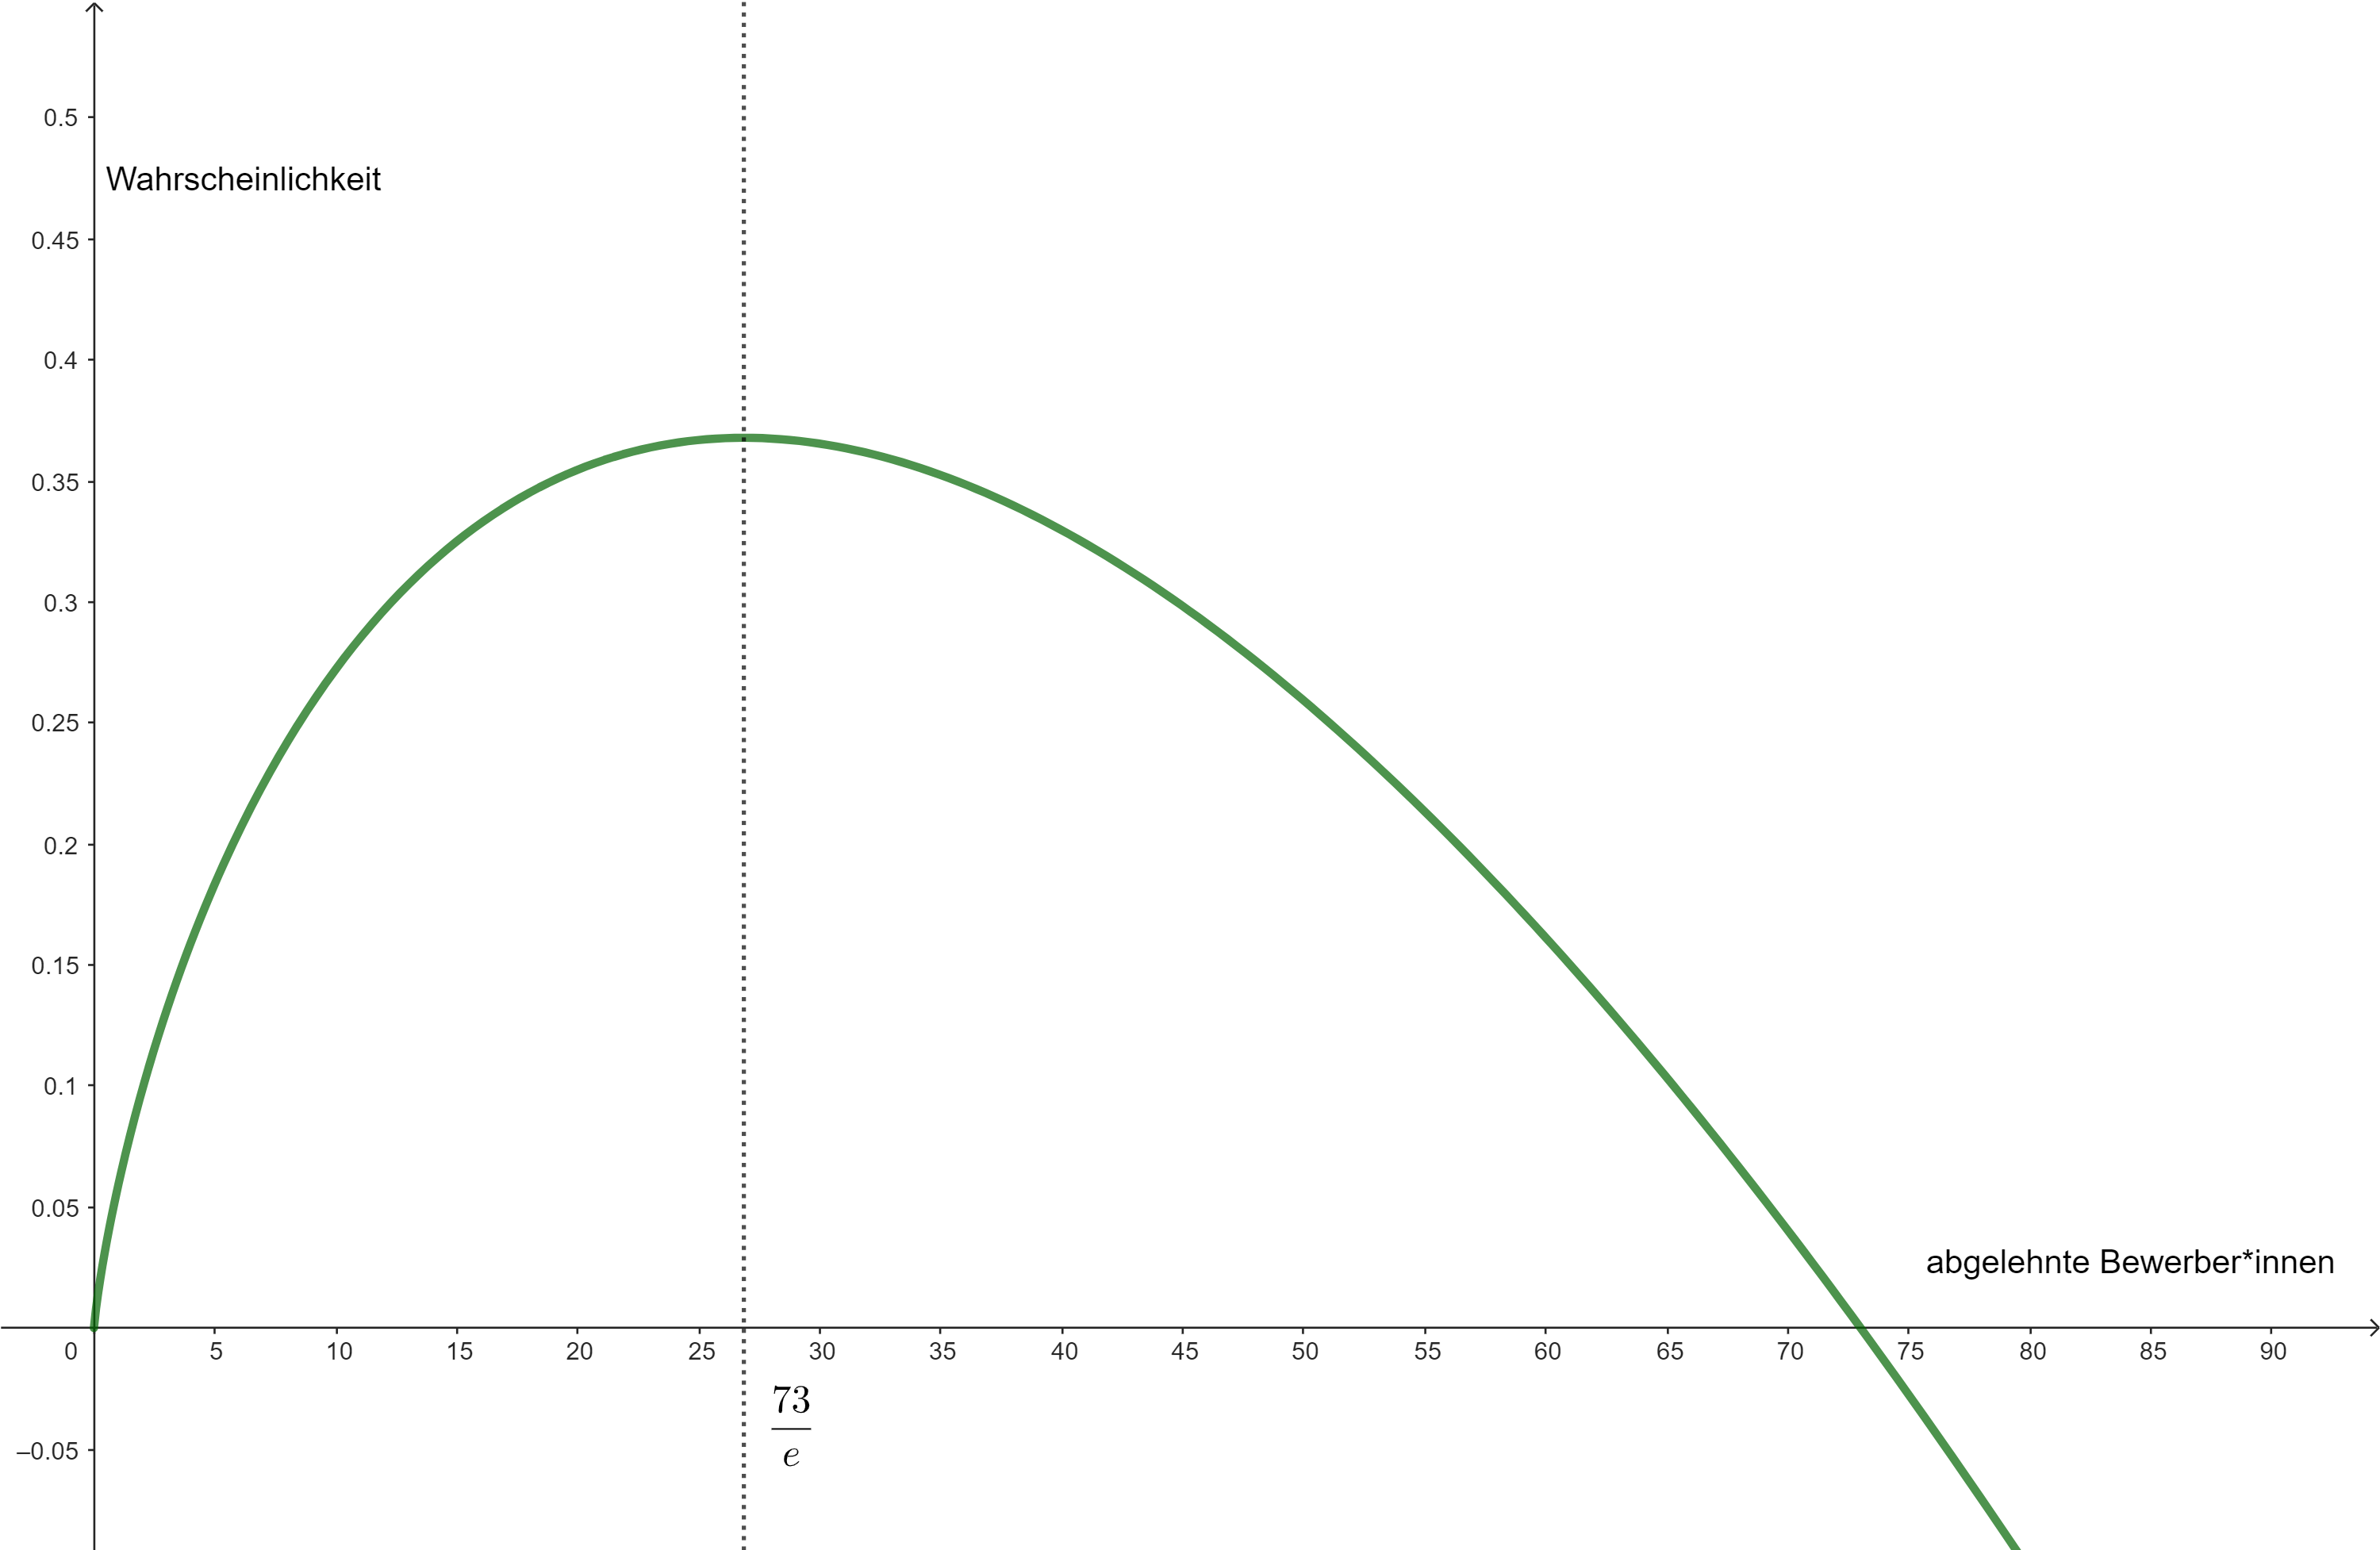
\includegraphics{images/wg/maximum.png}
Graph der Funktion $−\frac{x}{73}\ln⁡\left(\frac{x}{73}\right)$

"Ah, es gibt ein Maximum bei unserem $r$. Das heißt, für $r=\frac Ne$​ ist die Erfolgswahrscheinlichkeit unserer Strategie maximal", meint Maryam.

"Das stimmt nicht ganz.", entgegnet Bertrand, "wir haben die Summe ja nicht genau bestimmt sondern nur abgeschätzt. Außerdem können wir $r$ in Echt nur als ganze Zahl wählen, aber bei uns ist 
\[\frac{N}{e}=\frac{73}{e}\approx 26{,}86.\]
Wir können nicht $26{,}86$ Personen ablehnen, sondern nur $26$ oder $27$."

"Ok, alles ist nur abgeschätzt. Aber was ist denn nun die Wahrscheinlichkeit, dass die Strategie funktioniert, wenn wir $r=\frac{N}{e}$​ wählen?", fragt Maryam.
\[P(r)\approx -\frac rN \ln\left(\frac rN\right)\approx -\frac{N}{eN}\ln\left( \frac{N}{eN}\right)=-\frac 1e\ln\left(\frac 1e\right)=\frac 1e\approx 36{,}79\%\]
"Wow, also mit einer Wahrscheinlichkeit von ungefähr $36{,}79\%$ finden wir mit der Strategie die beste Person!", ruft Carl.

Quellen:
\begin{itemize}
	\item Abb. 1: zugeschnittenes Bild \href{https://commons.wikimedia.org/wiki/File:Lefthand-Reimann-Sum-Integral-Test.svg}{Lefthand-Riemann-Sum-Integral-Test von Lazauya}, \href{https://creativecommons.org/licenses/by-sa/4.0/}{CC BY-SA 4.0}, via Wikimedia Commons
\end{itemize}

\section{Anwendung der Strategie}
Emmy, Maryam, Carl und Bertrand sind mit ihrer Strategie zufrieden und beschließen, sie auszuprobieren. Für ihre $N=73$ Bewerber*innen wollen sie zunächst $\frac{N}{e}\approx 27=r$ Castings durchführen. Bertrand hat schon eine Tabelle vorbereitet, in der sie festhalten können, ab welchem \href{https://de.wikipedia.org/wiki/Scoville-Skala}{Scoville-Grad} jede dieser 27 Personen zu weinen anfängt.

27 Castings später haben sie die folgende Tabelle:
 \begin{tabular}{l|l|l}
	\textbf{Nr.} & \textbf{Name} & \textbf{Beginnt zu weinen bei einem Scoville-Grad von ...} \\\hline
	\hline
	1 & Constantin & 5.000 \\\hline
	2 & Sophie & 500 \\\hline
	3 & Alexander & 10.000 \ldots\\\hline
	$\vdots$ & $\vdots$ & $\vdots$\\\hline
	27 & Peter & 2.500\ldots\\\hline
\end{tabular}

Unter den 27 Castings war Alexander der beste Kandidat mit 10.000 Scoville. Von nun an werden alle Bewerber*innen mit diesem Ergebnis verglichen. Und in der Tat: Pierre-Simon, der 42. Bewerber, schlägt dieses Ergebnis mit beeindruckenden 20.000 Scoville. Mit (nicht nur Freuden-)Tränen in den Augen empfängt er die Nachricht, dass er ab nächstem Monat das Zimmer beziehen kann.

\section{Einordnung und Ausblick}
Die Aufgabe, aus einer Reihe einzeln betrachteter Bewerber den besten auszuwählen, wird “\href{https://de.wikipedia.org/wiki/Sekret%C3%A4rinnenproblem}{Sekretärinnenproblem}” oder auch “Heiratsproblem” genannt. Es hat Verbindungen in die Statistik, Spieltheorie und Entscheidungstheorie.

Die von Emmy, Maryam, Carl und Bertrand gewählte Strategie nennt man “\textbf{1/e-Regel}” oder “$37\%$-Regel”. Dabei schaut man sich zunächst $\frac 1e\approx37\%$ der Bewerbungen an und akzeptiert danach die erste Person, die besser als alle bisherigen ist. Wir haben gesehen, dass die Wahrscheinlichkeit, auf diese Weise die beste Person zu wählen, mindestens $\frac1e\approx 37\%$ beträgt.

Die 1/e-Regel ist sogar \textbf{optimal}: Es gibt keine Strategie, die eine größere Erfolgswahrscheinlichkeit hat. Das kann man mithilfe des \href{https://de.wikipedia.org/wiki/Odds-Strategie}{Odds-Algorithmus} zeigen, der im Jahr 2000 von \href{https://en.wikipedia.org/wiki/Franz_Thomas_Bruss}{Franz Thomas Bruss} entwickelt wurde. Das Sekretärinnenproblem ist ein Spezialfall davon.

Bruss hat außerdem 1984 das "\href{https://de.wikipedia.org/wiki/Sekret%C3%A4rinnenproblem#1/e-Gesetz_der_besten_Wahl}{1/e-Gesetz der besten Wahl}" bewiesen. Man sollte es nicht mit der “1/e-Regel” verwechseln, die Emmy, Maryam, Carl und Bertrand verwendet haben: Das 1/e-Gesetz der besten Wahl ist wesentlich allgemeiner. Es ist auch in nicht-diskreter Zeit und bei einer unbekannten Anzahl von Kandidaten anwendbar.

%%% Local Variables:
%%% mode: LaTeX
%%% TeX-master: "../../mfnf"
%%% End:
